\section{Principes de DICOM}

	\subsection{Objectifs de DICOM}
	
	\frame
	{
		\frametitle{Buts globaux}
		\begin{itemize}
			\item Trouver un langage commun pour l'\'echange (images et donn\'ees pertinentes) entre \'equipements d'imagerie : mettre en place un standard.
			\item Pousser les vendeurs \`a supporter ce langage commun.
			\item Standardiser :
			\begin{itemize}
				\item le stockage (i.e. format de fichier) ;
				\item et la communication des donn\'es (i.e. protocoles de communication).
			\end{itemize}
		\end{itemize}
	}
	
	\frame
	{
		\frametitle{Buts pr\'ecis}
		
		Il faut que lors de l'installation d'une nouvelle modalit\'e, le DICOM permette, sans changement d'un quelconque composant logiciel :
		\begin{itemize}
			\item l'interrogation du PACS ;
			\item la r\'ecup\'eration des images cr\'e\'ees par d'autres syst\`emes ;
			\item l'affichage des images ;
			\item et la production d'images lisibles par les syst\`emes d'autres constructeurs.
		\end{itemize}
	}

	\subsection{Fondements th\'eoriques}

	\frame
	{
		\frametitle{Monde r\'eel}
		Au cours d'un suivi m\'edical, un patient se voit prescrire des examens radiologiques par son m\'edecin.
		
		On peut sch\'ematiser la proc\'edure comme suit :
		
		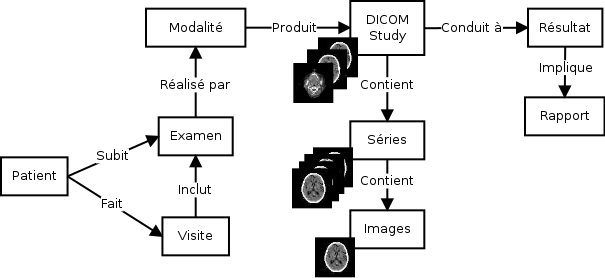
\includegraphics[width=\linewidth]{./figures/scenario.png}
		
		DICOM d\'ecrit ces donn\'ees et relations.
		
		La pr\'ecision du contenu et des liens d\'epend des outils et des utilisateurs (e.g. RIS et PACS).
	}

	\frame
	{
		\frametitle{Traduire le r\'eel en num\'erique}
		
		Un objet DICOM combine donc :
		\begin{itemize}
			\item des donn\'ees, ou informations (e.g. nom du patient, donn\'ees de l'image,?) ;
			\item et services, ou fonctions (e.g. sauvegarder, imprimer,?).
		\end{itemize}
		
		Le traitement DICOM d'une information consiste alors \`a regrouper :
		\begin{itemize}
			\item un \emph{Objet}, contenant les informations, se conformant \`a une \emph{Information Object Definition} (ou \emph{IOD}) ;
			\item et une fonction sp\'ecifique, ou \emph{Service}, se conformant \`a un \emph{DICOM Message Service Element}, ou \emph{DIMSE}.
		\end{itemize}
	}
	
	\frame
	{
		\frametitle{SOP Class UID}		

		La combinaison Objet + Service est :
		\begin{itemize}
			\item appel\'ee \emph{Service/Object Pair} ou \emph{SOP} ;
			\item l'\'el\'ement principal de la conformit\'e \`a la norme ;
			\item identifi\'ee par un identifiant unique nomm\'e \emph{SOP Class UID}.
		\end{itemize}
		
		Exemples de SOP Class UID :
		\begin{description}
			\item[$1.2.840.10008.5.1.4.1.1.1$] CR Image Store (sauvegarder  une image CR) ;
			\item[$1.2.840.10008.5.1.4.1.1.2$] CT Image Store (sauvegarder  un CT).
		\end{description}
	}
	
	\frame
	{
		\frametitle{Sch\'ema de construction du SOP}
		\begin{center}
			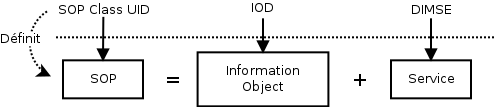
\includegraphics[width=\linewidth]{./figures/sop-definition.png}
		\end{center}		
	}